\documentclass{beamer}
\usepackage[spanish]{babel}
\usepackage{multicol}
\usepackage{neuralnetwork}
\usetheme{Warsaw}
\usecolortheme{crane}
\useoutertheme{shadow}
\useinnertheme{rectangles}

\setbeamertemplate{navigation symbols}{}

\title[Algoritmos y Estructura de datos]{Práctica 1: Algoritmos de ordenamiento}
\subtitle{Universidad Nacional de San Agustín}
\author{Christian Barriga Marcapura\\
        Weimar Ccapatinta Huamani}

\institute[Universidad Nacional de San Agustín]
{
  Universidad Nacional de San Agustín\\
    \and
    Seminario de Tesis\\
   \and
}
\date{20 de Agosto de 2022}

\AtBeginSection{
\begin{frame}
  \frametitle{Índice}
  \tableofcontents[currentsection]  
\end{frame}
}
\begin{document}

\begin{frame}
  \frametitle{Índice}
  \tableofcontents
\end{frame}

\section{Introducción}
\begin{frame}
  \frametitle{Introducción}
  \begin{block}{}
El análisis de algoritmos puede entenderse como la estimación del consumo de recursos que un algoritmo requiere, proporcionando herramientas para poder estimar si una solución propuesta satisface las restricciones de recursos de un problema sin necesidad de implementarlo.
  \end{block}
    \begin{block}{}
  En la práctica 1 vamos a realizar un análisis cuatro algoritmos de ordenamiento con tres tipos de programación, obteniendo de esta manera un cuadro comparativo, del cual a partir de ello evaluaremos que tipo de lenguaje es mucho mas funcional respecto al algoritmo probado, para tal motivo se esta utilizando el mismo ordenador, asi como editor de texto para poder mantener las mismas condiciones para los diversos tipos de lenguaje.
  \end{block}
\end{frame}

\section{Algoritmos}

\subsection{Merge sort}
\begin{frame}
 \frametitle{Merge sort}
    \begin{block}{}
Algoritmo basado en la técnica DyV
\begin{itemize}
    \item Divide el vector en dos partes iguales.
    \item Ordena por separado cada una de las partes (llamando recursivamente a ordenaPorFusión).
    \item mezcla ambas partes manteniendo la ordenación.
\end{itemize}
  \end{block}  
\end{frame}
\begin{frame}
 \frametitle{Merge sort}
    \begin{block}{}
\textbf{Algoritmo Merge Sort}\\
\definecolor{Micolor1}{RGB}{45,87,44}
\newcommand\tab[1][1cm]{\hspace*{1}}
\textcolor{Micolor1}{
\tab dividir cada elemento en particiones de tamaño 1\\
\tab fusionar recursivamente particiones adyacentes\\}
\tab for i = leftPartIdx to rightPartIdx\\
\tab \tab   if leftPartHeadValue <= rightPartHeadValue\\
\tab \tab \tab      copy leftPartHeadValue\\
\tab \tab    else: copy rightPartHeadValue; Increase InvIdx\\
\textcolor{Micolor1}{
\tab copiar elementos de nuevo a la matriz original}
  \end{block}  
\end{frame}
  
  \begin{frame}
 \frametitle{Merge sort}
    \begin{block}{}
\textbf{Costo Computacional}\\
La longitud de la Lista es N\\
Dos listas N/2\\
El tiempo a*N\\
Suposición $N = 2^k$

Cuando la lista es pequeña  $T(1) = T(0)= b$\\
$T(N) = 2* T(N/2) + a* N$

$k = log2 N$\\
En consecuencia
\begin{equation}
T(N)\equiv b*N+a*N*Log2 N
\end{equation}
\end{block} 
\end{frame}

\subsection{Quick sort}
  \begin{frame}
 \frametitle{Quick sort}
    \begin{block}{}
Es un algoritmo DyV muy parecido al de la selección (búsqueda del k-ésimo menor elemento):
\begin{itemize}
    \item se reorganiza la tabla en dos subtablas respecto a un pivote: elementos mayores o iguales a un lado y menores al otro, después de la reorganización, el pivote ocupa exactamente el lugar que le corresponderá en la lista ordenada
    \item se repite el proceso de forma recursiva para cada subtabla
\end{itemize}
  \end{block}  
\end{frame}
\begin{frame}
 \frametitle{Quick sort}
    \begin{block}{}
\textbf{Algoritmo Quick Sort}\\

\tab para cada partición (sin ordenar)\\
\tab establecer el primer elemento como pivote\\
\tab\tab   storeIndex = pivotIndex+1\\
\tab\tab   for i = pivotIndex+1 to rightmostIndex\\
\tab\tab\tab     if ((a[i] < a[pivot]) o (igual pero 50p/ciento afortunado))\\
\tab\tab       swap(i, índicetienda); ++storeIndex\\
\tab   intercambio (pivote, storeIndex-1)\\
  \end{block}  
\end{frame}
  \begin{frame}
 \frametitle{Quick sort}
    \begin{block}{}
\textbf{Costo Computacional}\\
Su tiempo es menor que e de todos los algoritmos de ordenación de complejiad O(n log n)
\begin{center}
   \begin{tabular}{|c|c|c|}
\hline 
\textbf{Pivote} & \textbf{Peor caso} & \textbf{Caso Promedio}\tabularnewline
\hline 
primer elemento & \textbf{O($n^2$)} & O(n log n)\tabularnewline\hline 
intermedio de los elementos & \textbf{O($n^2$)} & O(n log n)\tabularnewline\hline 
pseudo-mediana & O(n log n) & O(n log n)\tabularnewline\hline 
\end{tabular} 
\end{center}
Podemos imaginar un comportamiento parecido al Merge sort\\
$T(N) \equiv N * log2 N$
  \end{block}  
\end{frame}
\subsection{Insertion sort}
  \begin{frame}
 \frametitle{Insertion sort}
    \begin{block}{}
Este algoritmo divide la tabla en una parte ordenada y otra no
\begin{itemize}
    \item la parte ordenada comienza estando formada por un único elemento (el que ocupa la primera posición de la tabla)
    \item los elementos son insertados uno a uno desde la parte no ordenada a la ordenada
    \item finalmente la parte ordenada acaba abarcando toda la tabla
\end{itemize}
  \end{block}  
\end{frame}
 \begin{frame}
 \frametitle{Insertion sort}
    \begin{block}{}
\textbf{Algoritmo Insertion Sort}\\
\tab marcar el primer elemento como ordenado\\
\tab para cada elemento sin clasificar X\\
\tab \tab    'extraer' el elemento X\\
\tab \tab    for j = lastSortedIndex hasta 0\\
\tab \tab \tab      if elelemento actual j > X\\
\tab \tab \tab        mover elemento ordenado a la derecha por 1\\
\tab \tab      romper bucle e insertar X aquí\\
  \end{block}  
\end{frame}
  \begin{frame}
 \frametitle{Insertion sort}
    \begin{block}{}
\textbf{Costo Computacional}\\
\begin{equation}
C(n-1+1)((n-1)/2)=cn^2/2-cn/2
\end{equation}
Al utilizar una notación grande, podemos descartar $cn/2$\\
El peor caso se da cuando la tabla se encuentra inicialmente ordenada en orden decreciente
\begin{equation}
T(n)=\theta(n^2)
\end{equation}
Cuando la tabla esta ordenada su tiempo de ejecución es:
\begin{equation}
T(n)= \theta(n)
\end{equation}
  \end{block}  
\end{frame}
\subsection{Radix sort}
 \begin{frame}
 \frametitle{Radix sort}
    \begin{block}{}
Es una generalización del método de ordenación por cajas\\
\begin{itemize}
    \item Se crea una cola para cada dígito
    \item Se encola cada elemento en la cola correspondiente a su dígito menos significativo
    \item Se vuelcan los contenidos de las colas en el array
    \item Se vuelven a encolar, ahora en base a su segundo dígito menos significativo y así sucesivamente
\end{itemize}
  \end{block}  
\end{frame}
\begin{frame}
 \frametitle{Radix sort}
    \begin{block}{}
\textbf{Algoritmo Radix Sort}\\
\tab crear 10 cubos (colas) para cada dígito (0 a 9)\\
\tab por cada digito colocado\\
\tab   para cada elemento en la lista\\
\tab \tab     mover el elemento al cubo respectivo\\
\tab   para cada cubo, a partir del dígito más pequeño\\
\tab \tab     mientras el cubo no está vacío\\
\tab \tab      restaurar elemento a la lista\\
  \end{block}  
\end{frame}
 \begin{frame}
 \frametitle{Radix sort}
    \begin{block}{}
\textbf{Costo Computacional}\\
Análisis de eficiencia\\
• El lazo externo se realiza k veces\\
• El primer lazo se realiza n veces\\
• Los lazos anidados para volcar las cajas en el array se realizan\\
en el peor caso b+n-1 veces (O(n) cuando b$<<$n)\\
• Luego su eficiencia es O(k*n)
  \end{block}  
\end{frame}
\section{Resultados}
\begin{frame}
 \frametitle{Resultados}
    \begin{block}{}
\center\includegraphics[trim={0.1cm 0.2cm 0cm 0.6cm},clip,scale=0.31]{Tiempo de Procesamiento vs Tamaño de lista 1.png}
\center Figura 1 Tiempo de procesamiento vs Tamaño de Lista - Elaboración propia
  \end{block}
 \end{frame}
\begin{frame}
  \frametitle{Resultados}
  \begin{block}{}
\center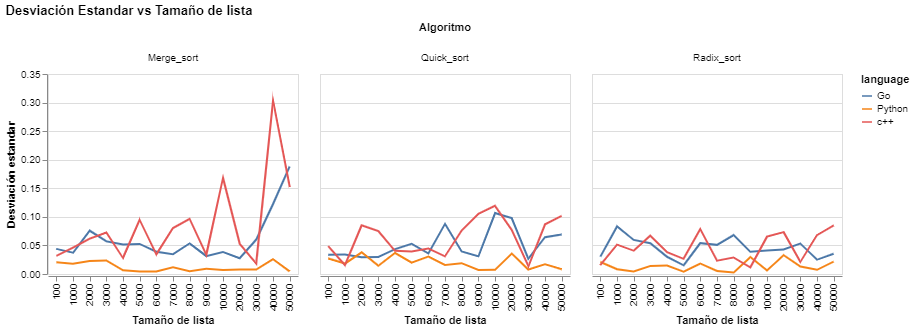
\includegraphics[trim={0.1cm 0.2cm 0cm 0.6cm},clip,scale=0.31]{SDvsTL.png}
\center Figura 2 Desviación Standard vs Tamaño de Lista - Elaboración propia
  \end{block}
\end{frame}
\begin{frame}
 \frametitle{Resultados}
    \begin{block}{}
\center\includegraphics[trim={0.1cm 0.2cm 0cm 0.6cm},clip,scale=0.31]{Tiempo de Procesamiento vs Tamaño de lista x lenguaje de prog.png}
\center Figura 3 Tiempo de procesamiento vs Tamaño de Lista - Lenguaje de Programación - Elaboración propia
  \end{block}
 \end{frame}
 \begin{frame}
 \frametitle{Resultados}
    \begin{block}{}
\center\includegraphics[trim={0.1cm 0.2cm 0cm 0.6cm},clip,scale=0.31]{Tiempo de Procesamiento vs Tamaño de lista 2.png}
\center Figura 4 Tiempo de procesamiento vs Tamaño de Lista - Elaboración propia
  \end{block}
 \end{frame}
\section{Conclusiones}
\begin{frame}
  \frametitle{Conclusiones}
\doublespacing\begin{itemize}
  \item El algoritmo que tuvo mejor resultado fue el Radix sort y en el lenguaje de ería el python.
  \item En las pruebas realizadas se puede considerar como mejor algoritmo el radix siendo casi similar a los demas algoritmos a excepción de Insert que tiene un costo de $n^2$
  \item El lenguaje a parte de su sencillez para programar tiene los tiempos mas bajos a excepción del modelo Insert, ademas tiene poca variabilidad en sus tiempos. 
\end{itemize}
\end{frame}
 \end{document}